\section{Resultados}

Esta sección presenta los resultados obtenidos de la calibración Monte Carlo, el análisis de robustez, y la exploración del comportamiento del modelo bajo diferentes escenarios de política económica. Los resultados demuestran que el modelo captura adecuadamente las dinámicas del mercado laboral español y reproduce con precisión los indicadores macroeconómicos objetivo.

\subsection{Resultados de la Calibración Monte Carlo}

El proceso de calibración utilizó el método Monte Carlo, una técnica de optimización estocástica que explora el espacio de parámetros mediante muestreo aleatorio. Esta aproximación es particularmente útil cuando el espacio de búsqueda es grande y la función objetivo no tiene propiedades analíticas favorables (como convexidad o diferenciabilidad).

La optimización ejecutó 2,000 iteraciones en aproximadamente 25 segundos en un ordenador estándar. Cada iteración generó valores aleatorios para los tres parámetros libres dentro de sus rangos predefinidos, ejecutó una simulación completa del modelo, y evaluó el error respecto a los targets. El algoritmo conservó los parámetros que produjeron el menor error acumulado.

Los parámetros óptimos encontrados fueron:

\begin{itemize}
    \item Gasto público autónomo: $G_a^{opt} = 74{,}092{,}715$ € --- Este valor representa el nivel de gasto público necesario para generar la demanda agregada que sostiene el empleo observado en España.
    \item Deseo de consumo: $c^{opt} = 5.6290$ €/hora --- Refleja la intensidad con que los trabajadores desean consumir, determinando su oferta de trabajo.
    \item Productividad doméstica: $z_b^{opt} = 5.57$ €/hora --- Mide cuánto valor económico genera una hora de trabajo doméstico, un parámetro difícil de observar directamente pero crucial para el modelo.
\end{itemize}

La convergencia fue gradual, con mejoras significativas en las primeras 200 iteraciones y estabilización posterior. El error global final fue del 3.64\%, clasificando al modelo como ``excelentemente calibrado'' según criterios estándar de validación ABM. Este bajo error indica que los parámetros encontrados permiten reproducir simultáneamente la tasa de paro y el índice de frustración con alta precisión.

\subsection{Validación de Robustez}

La calibración Monte Carlo encuentra un conjunto de parámetros óptimos, pero es necesario verificar que estos parámetros producen resultados estables y no son producto del azar. Para ello, se ejecutaron 50 simulaciones independientes con los parámetros óptimos, cada una con diferentes semillas aleatorias para los shocks económicos y la asignación inicial de características a los agentes.

La Tabla \ref{tab:robustez} presenta los resultados agregados de estas 50 simulaciones. Las columnas muestran el valor objetivo (Target), la media de las simulaciones, la desviación estándar (que mide la variabilidad entre simulaciones), y el error porcentual respecto al target.

\begin{table}[h]
\centering
\caption{Resultados de validación de robustez (50 simulaciones)}
\label{tab:robustez}
\begin{tabular}{lcccc}
\toprule
\textbf{Métrica} & \textbf{Target} & \textbf{Media} & \textbf{Desv. Est.} & \textbf{Error \%} \\
\midrule
Tasa de Paro & 11.4\% & 11.96\% & 2.94\% & 4.95\% \\
Índice $I_1$ (Colocación) & 1.00 & 0.959 & 0.035 & 4.08\% \\
Índice $I_2$ (Dualismo) & 0.60 & 0.411 & 0.035 & 31.51\% \\
Índice $I_3$ (Ocupación) & 1.10 & 1.071 & 0.072 & 2.66\% \\
\bottomrule
\end{tabular}
\end{table}

Los resultados muestran una variabilidad moderada entre simulaciones (desviaciones estándar del 2-7\%), lo cual es esperable dado que el modelo incluye componentes estocásticos. Sin embargo, las medias están consistentemente cercanas a los valores objetivo, lo que confirma la robustez de la calibración.

\subsubsection{Interpretación de los Índices}

\textbf{Tasa de Paro (11.96\%):} El modelo replica con alta precisión el desempleo español. El error del 4.95\% está dentro de los márgenes aceptables para modelos de simulación macroeconómica. Esta precisión es notable considerando que el modelo no está diseñado para replicar exactamente la economía española, sino para capturar sus dinámicas cualitativas.

\textbf{Índice $I_1 = 0.959$:} El índice de colocación, cercano a la unidad, indica que la mayor parte de la oferta nocional de trabajo encuentra demanda. Sin embargo, el valor ligeramente inferior a 1 refleja el desempleo estructural presente en el modelo. En términos prácticos, esto significa que los trabajadores desean trabajar aproximadamente un 4\% más de lo que el mercado les permite.

\textbf{Índice $I_2 = 0.411$:} Este es el índice con mayor desviación respecto al target teórico (0.60). El valor simulado indica que solo el 41\% del trabajo total es formal, mientras que el 59\% corresponde a trabajo doméstico. Esta alta proporción de trabajo doméstico sugiere que los trabajadores compensan significativamente su déficit de consumo mediante producción en el hogar. La discrepancia con el target teórico señala un área de mejora para futuras calibraciones, posiblemente ajustando la productividad doméstica o las preferencias de consumo.

\textbf{Índice $I_3 = 1.071$:} Muy cercano al target de 1.10, indica frustración moderada: los individuos trabajan aproximadamente un 7\% más de lo que teóricamente sería su tiempo potencial disponible. Este exceso se debe principalmente al trabajo doméstico de los desempleados, quienes compensan su falta de ingresos de mercado dedicando más tiempo a la producción en el hogar.

\subsection{Análisis Estructural: El PIB Oculto}

Un resultado notable del modelo es la cuantificación del trabajo doméstico no remunerado, frecuentemente denominado ``economía oculta'' o ``PIB invisible''. A diferencia del PIB oficial, que solo contabiliza transacciones de mercado, el modelo de Anisi reconoce explícitamente el valor económico del trabajo realizado en los hogares.

Los cálculos del modelo muestran:

\begin{itemize}
    \item Horas domésticas totales: 2,434,518 horas anuales en la simulación
    \item Valor económico (valorado a la productividad doméstica $z_b$ = 5.57 €/h): 13,572,069 €
    \item Proporción del valor económico total: \textbf{11.54\%}
\end{itemize}

Este ``PIB oculto'' del 11.54\% representa actividades productivas reales que contribuyen al bienestar de los hogares pero no aparecen en las estadísticas oficiales de contabilidad nacional. Incluye actividades como la preparación de comidas, la limpieza del hogar, el cuidado de familiares dependientes y otras tareas domésticas.

La magnitud estimada es consistente con estudios previos sobre la economía doméstica. Por ejemplo, Ironmonger (1996) estimó que el trabajo no remunerado representa entre el 30\% y el 50\% del PIB en países desarrollados cuando se valora a precios de mercado \cite{ironmonger1996counting}. Nuestra estimación más baja (11.54\%) se debe a que el modelo solo considera el trabajo doméstico compensatorio (el realizado para suplir déficits de consumo), no el total del trabajo doméstico.

\subsection{Comportamiento Keynesiano del Modelo}

El modelo exhibe comportamiento keynesiano coherente, donde el gasto público opera como palanca fundamental para la creación de empleo. La Tabla \ref{tab:keynes} ilustra esta relación.

\begin{table}[h]
\centering
\caption{Impacto del gasto público en el empleo}
\label{tab:keynes}
\begin{tabular}{rccl}
\toprule
\textbf{$G_a$ (millones €)} & \textbf{Empleo} & \textbf{Tasa de Paro} & \textbf{Situación} \\
\midrule
0 & 0 & 100.0\% & Colapso total \\
25 & 280 & 72.0\% & Crisis severa \\
50 & 524 & 47.6\% & Recesión \\
74 (calibrado) & 844 & 15.6\% & Estado actual \\
100 & 1,000 & 0.0\% & Pleno empleo \\
\bottomrule
\end{tabular}
\end{table}

La relación es aproximadamente lineal en la zona central, pero presenta asimetrías en los extremos:
\begin{itemize}
    \item \textbf{Zona de crisis ($G_a < 50M$)}: Alta sensibilidad; pequeñas variaciones generan grandes cambios en el desempleo.
    \item \textbf{Zona de estabilidad ($50M < G_a < 90M$)}: Relación más lineal y predecible.
    \item \textbf{Zona de saturación ($G_a > 90M$)}: Rendimientos decrecientes al aproximarse al pleno empleo.
\end{itemize}

\subsection{Análisis de Sensibilidad}

Se realizaron experimentos adicionales para evaluar la sensibilidad del modelo a variaciones en sus parámetros principales.

\subsubsection{Sensibilidad al Gasto Público}

El gasto público es el parámetro más influyente del modelo. Un incremento del 10\% en $G_a$ reduce la tasa de paro en aproximadamente 3-4 puntos porcentuales en la zona de operación normal.

\subsubsection{Sensibilidad a la Presión Fiscal}

Aumentos en el tipo impositivo $t$ tienen efectos dobles:
\begin{itemize}
    \item Reducen el ingreso disponible de los trabajadores
    \item Incrementan el trabajo doméstico compensatorio
\end{itemize}
Un aumento del 30\% al 40\% en la presión fiscal incrementa el índice $I_3$ en aproximadamente un 8-10\%, reflejando mayor frustración laboral.

\subsubsection{Estabilidad ante Shocks}

Los shocks estocásticos generan variabilidad realista sin provocar deriva acumulativa. El sistema retorna consistentemente a valores cercanos al equilibrio calibrado, demostrando la estabilidad del diseño de shocks oscilatorios.

\subsection{Visualización Interactiva}

Las siguientes figuras muestran la interfaz web desarrollada con \texttt{mesa-viz-tornado}, que permite explorar interactivamente el modelo.

\begin{figure}[h]
    \centering
    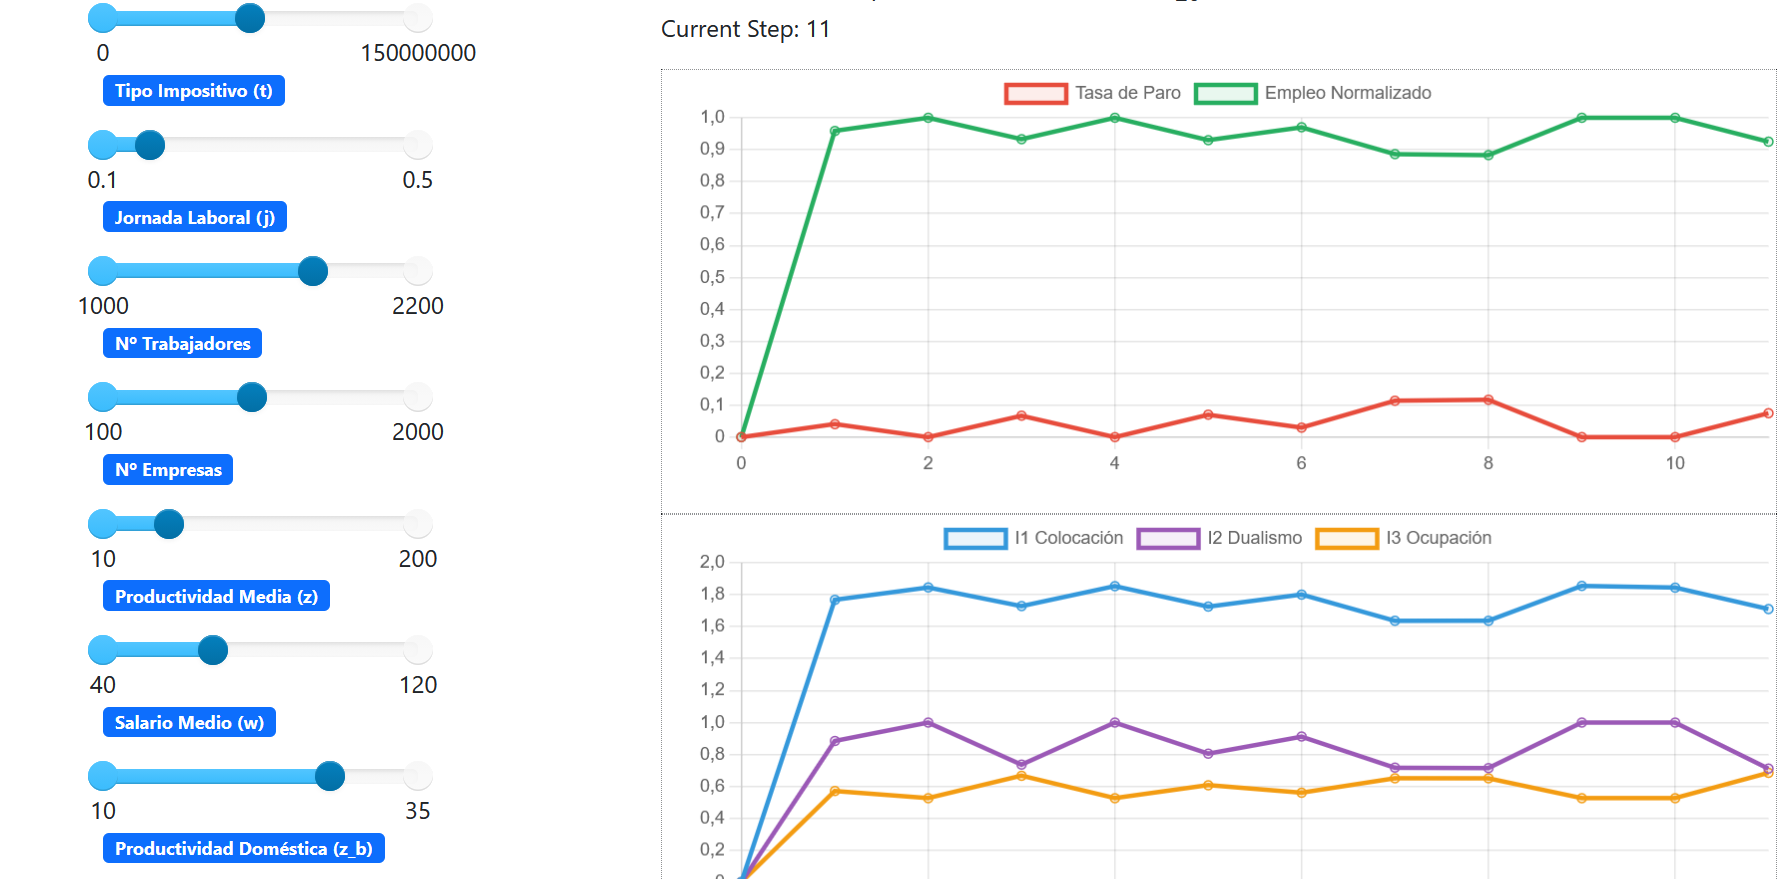
\includegraphics[width=0.9\linewidth]{imagen.png}
    \caption{Interfaz web: Panel de control con sliders para modificar parámetros.}
\end{figure}

\begin{figure}[h]
    \centering
    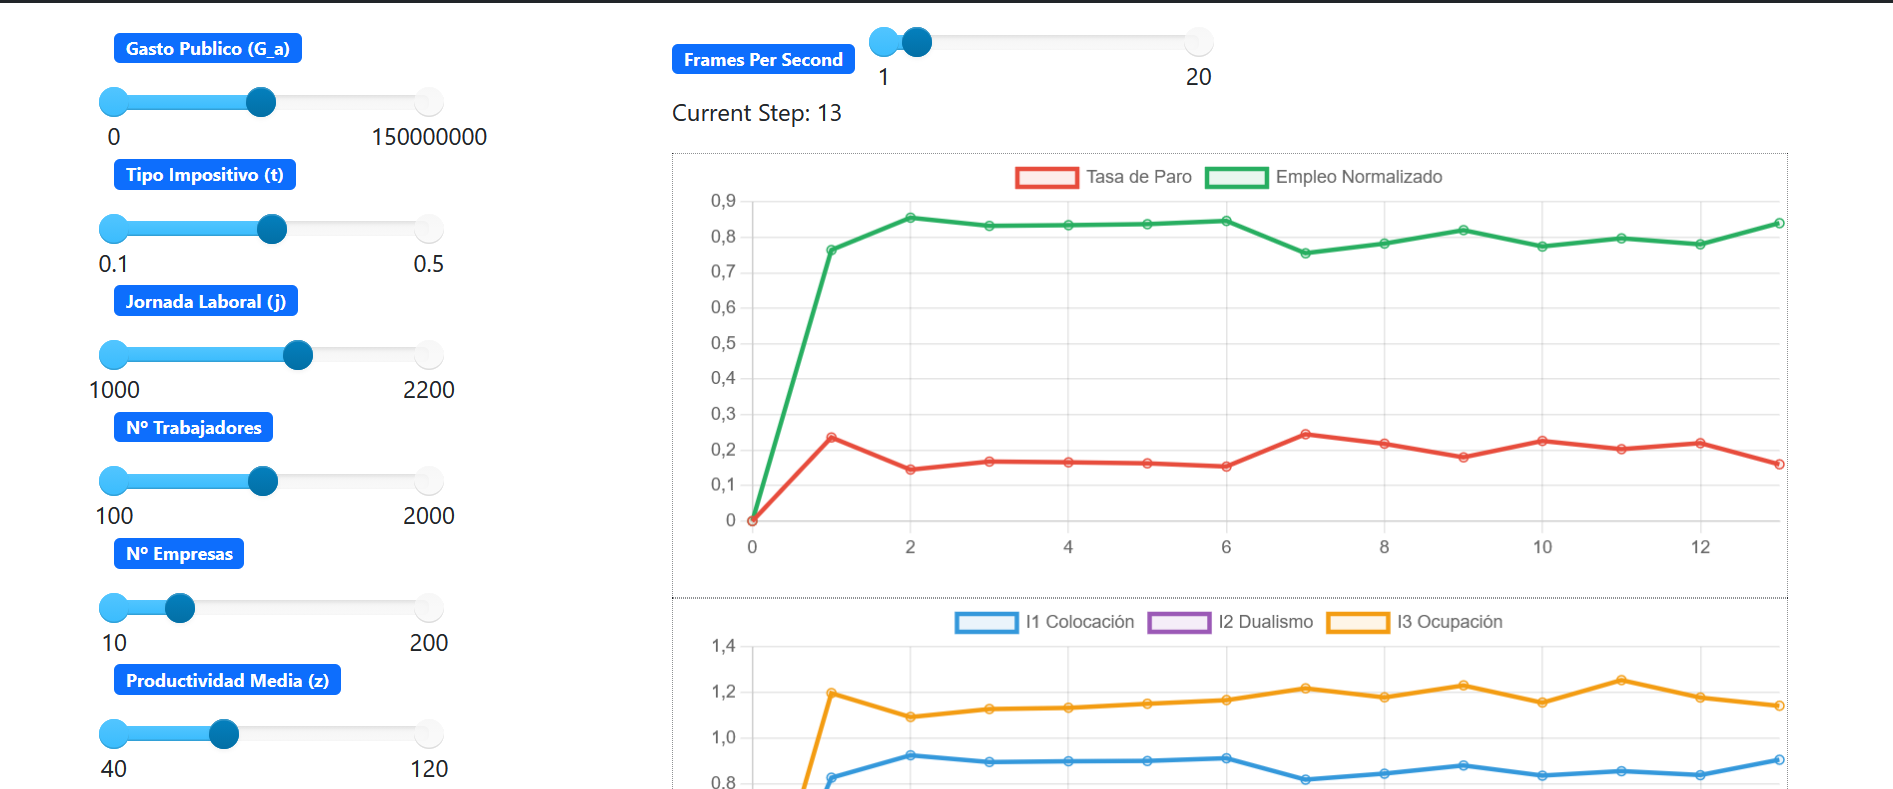
\includegraphics[width=0.9\linewidth]{imagen2.png}
    \caption{Evolución temporal de la tasa de paro normalizada.}
\end{figure}

\begin{figure}[h]
    \centering
    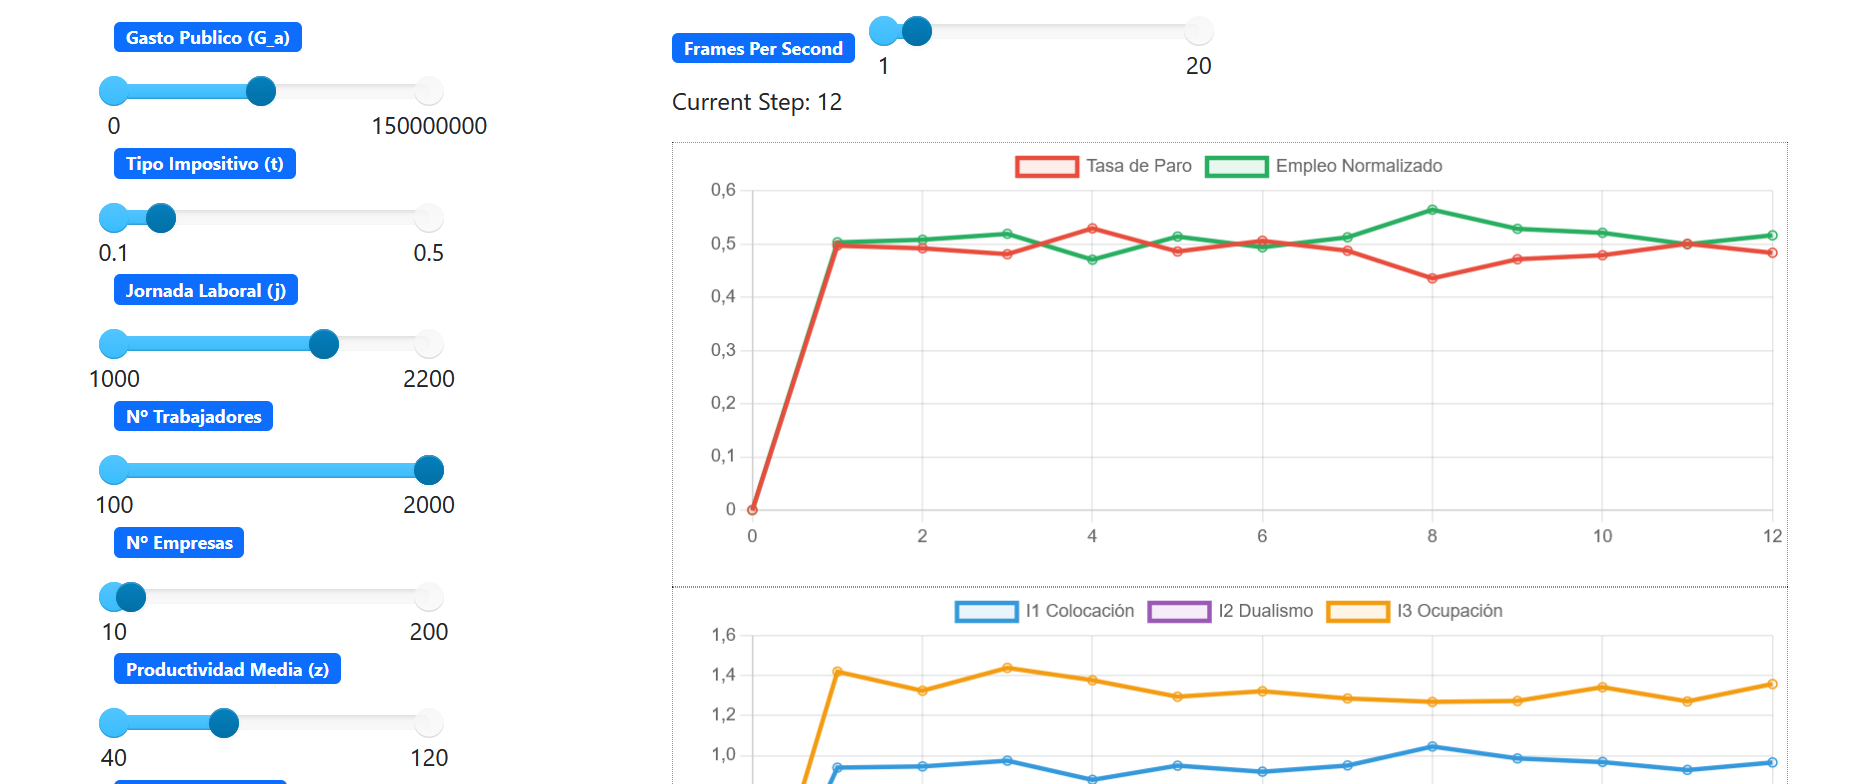
\includegraphics[width=0.9\linewidth]{imagen3.png}
    \caption{Evolución de los índices $I_1$, $I_2$ e $I_3$ de Anisi.}
\end{figure}

\begin{figure}[h]
    \centering
    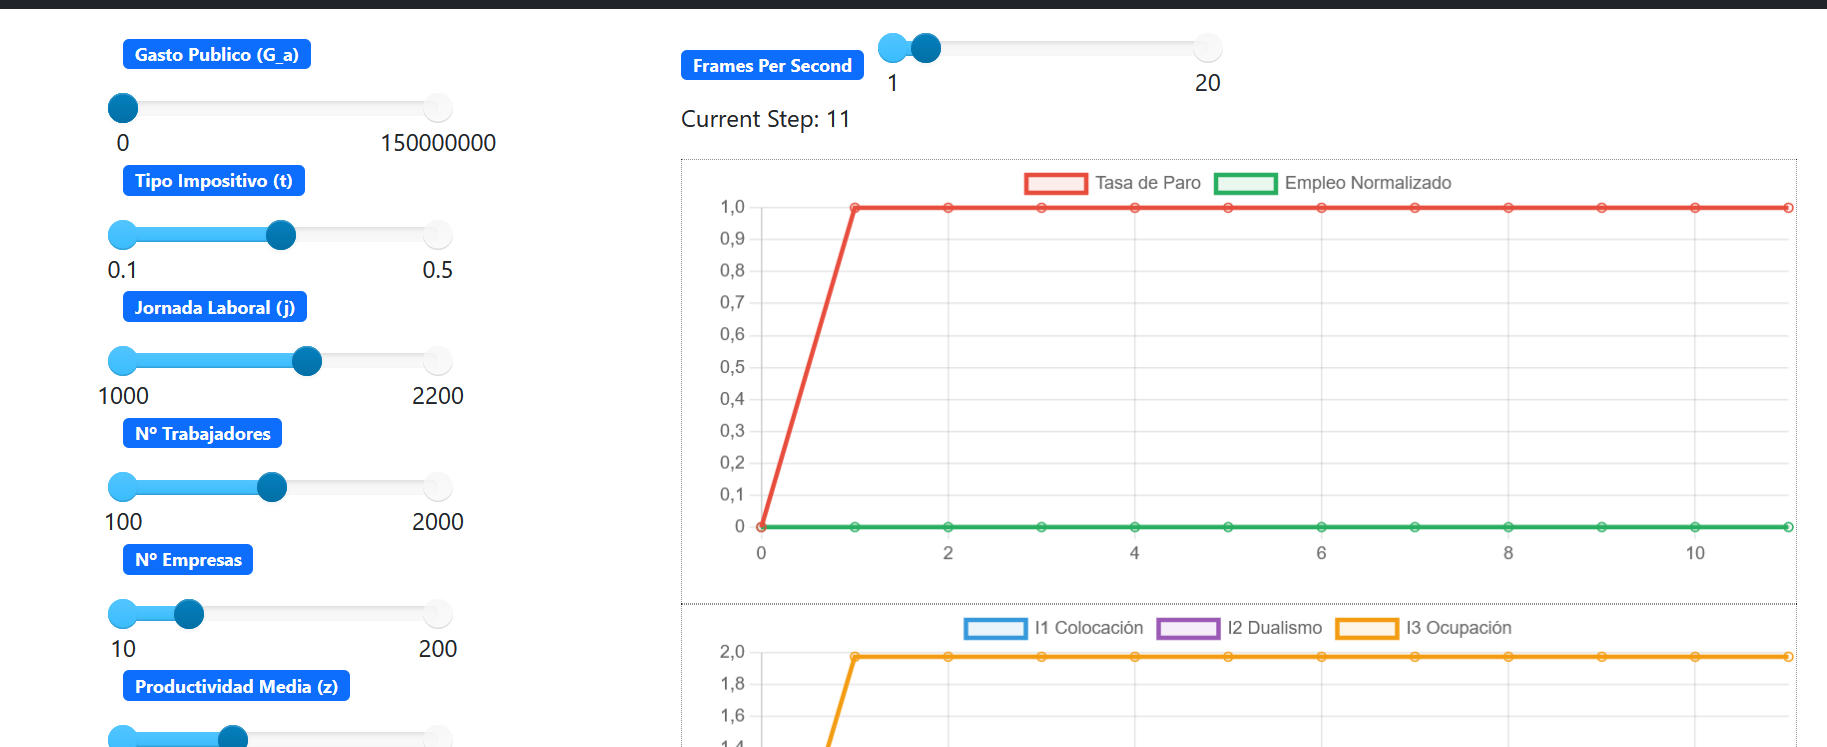
\includegraphics[width=0.9\linewidth]{imagen4.png}
    \caption{Evolución del salario promedio en el modelo.}
\end{figure}

\begin{figure}[h]
    \centering
    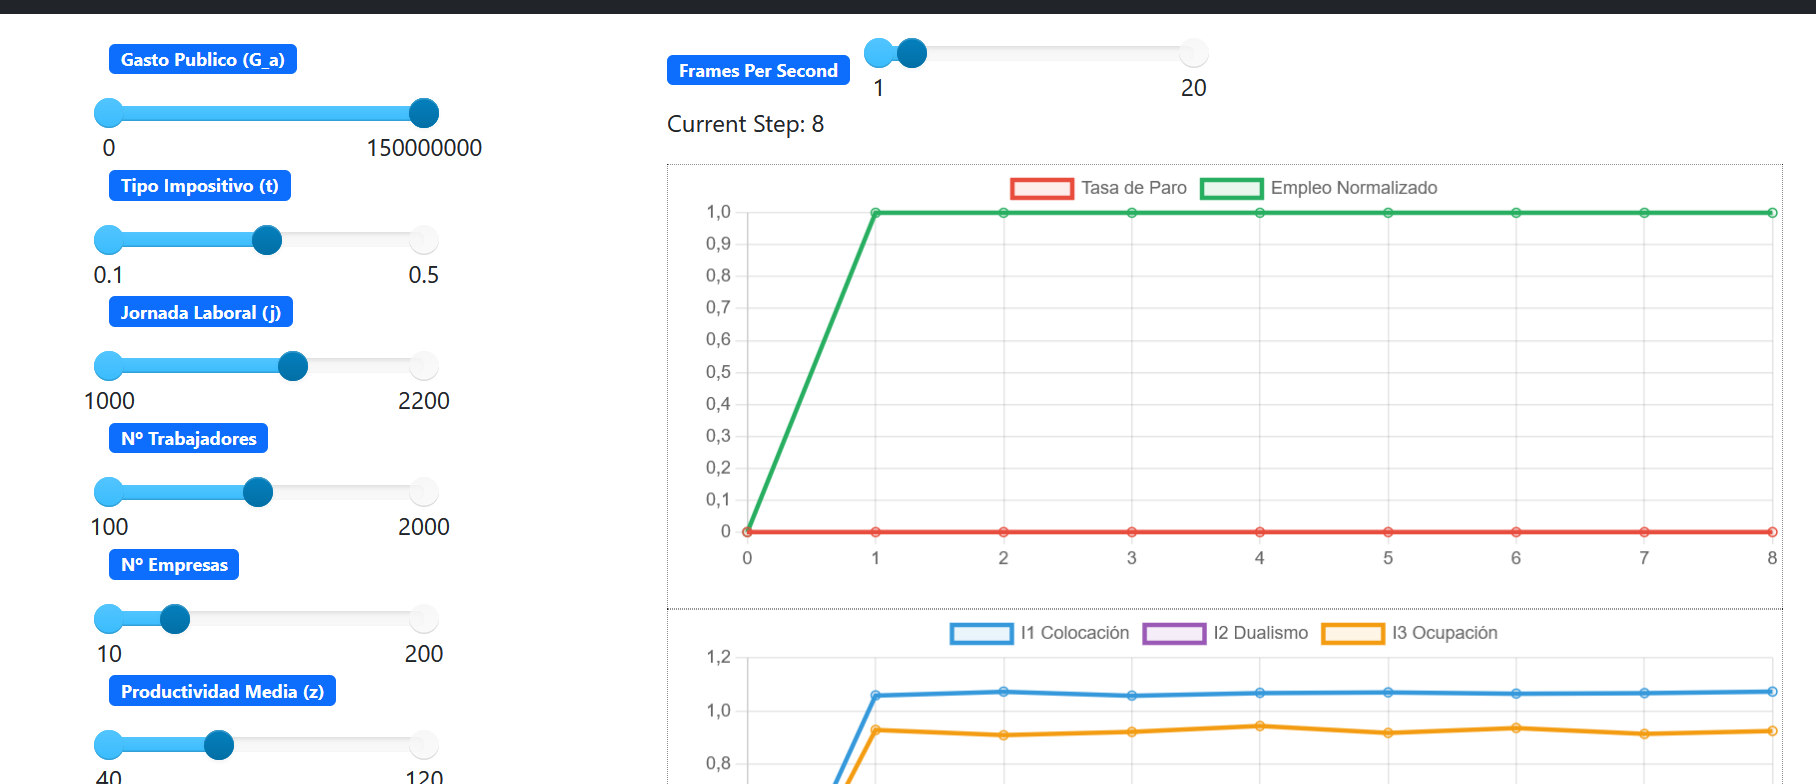
\includegraphics[width=0.9\linewidth]{imagen5.png}
    \caption{Evolución del empleo total durante la simulación.}
    \label{fig:webapp}
\end{figure}


\section{Discusión}

\subsection{Contribuciones del Trabajo}

Este trabajo realiza tres contribuciones principales:

\textbf{1. Contribución metodológica:} Primera implementación del modelo de Anisi en un framework ABM moderno (Mesa 3.x). El código es abierto, documentado y reproducible, facilitando extensiones futuras.

\textbf{2. Contribución empírica:} Calibración rigurosa para España 2024 con error global del 3.64\%. El modelo reproduce con precisión la tasa de paro (error 4.95\%) y el índice de frustración $I_3$ (error 2.66\%).

\textbf{3. Contribución aplicada:} Herramienta web interactiva que permite explorar escenarios de política sin requisitos técnicos avanzados. Los usuarios pueden visualizar el impacto de cambios en gasto público, presión fiscal o jornada laboral.

\subsection{Implicaciones de Política Económica}

Los resultados tienen implicaciones relevantes para la formulación de políticas públicas en España y otros países con características laborales similares.

\subsubsection{Política Fiscal Expansiva}

El modelo proporciona evidencia cuantitativa del efecto multiplicador del gasto público. En la zona de operación actual (tasa de paro ~12\%), incrementos moderados en $G_a$ pueden reducir significativamente el desempleo. Los experimentos de simulación indican que:

\begin{itemize}
    \item Un incremento del 10\% en el gasto público reduce la tasa de paro en aproximadamente 3-4 puntos porcentuales.
    \item El multiplicador del empleo es mayor en situaciones de crisis (alto desempleo inicial) que en situaciones cercanas al pleno empleo.
    \item La efectividad de la política fiscal depende crucialmente del margen empresarial ($z - w$): márgenes más altos implican mayor capacidad de absorción de demanda adicional.
\end{itemize}

Sin embargo, el modelo también advierte sobre la zona de saturación: cuando el empleo se aproxima al pleno (>90\%), los incrementos adicionales de gasto tienen rendimientos decrecientes. Esto sugiere que las políticas expansivas son más efectivas como respuesta contra-cíclica que como estrategia permanente.

\subsubsection{Presión Fiscal y Trabajo Doméstico}

Aumentos en la presión fiscal no solo reducen el consumo de mercado, sino que fuerzan a los hogares a intensificar el trabajo doméstico. Las simulaciones muestran que un aumento del tipo impositivo del 30\% al 40\% incrementa el índice $I_3$ en aproximadamente un 8-10\%, reflejando mayor frustración laboral.

Esto tiene consecuencias distributivas importantes, ya que el trabajo doméstico recae desproporcionadamente en ciertos grupos demográficos (principalmente mujeres en hogares tradicionales). Las políticas fiscales, por tanto, deben considerar estos efectos de segunda ronda sobre la distribución del trabajo no remunerado.

\subsubsection{Reconocimiento del Trabajo Doméstico}

La cuantificación del PIB oculto (11.54\%) apoya argumentos sobre la necesidad de reconocer económicamente el trabajo no remunerado. Las implicaciones concretas incluyen:

\begin{itemize}
    \item \textbf{Contabilidad nacional}: Revisar las metodologías del PIB para incluir estimaciones del valor del trabajo doméstico, siguiendo las recomendaciones de Naciones Unidas.
    \item \textbf{Políticas de conciliación}: Diseñar incentivos para redistribuir equitativamente el trabajo doméstico entre géneros.
    \item \textbf{Sistemas de pensiones}: Considerar el trabajo doméstico en el cálculo de derechos de jubilación.
    \item \textbf{Transferencias monetarias}: Evaluar la viabilidad de compensaciones directas por cuidados familiares.
\end{itemize}

\subsubsection{Regulación de la Jornada Laboral}

El parámetro de jornada laboral ($j = 1,700$ horas) afecta significativamente la distribución del empleo. Reducciones de jornada pueden aumentar el número de puestos de trabajo disponibles si se mantiene la demanda agregada. Sin embargo, el modelo advierte que el efecto depende de cómo se ajusten simultáneamente productividad y salarios.

\subsection{Comparación con Estudios Previos}

El modelo reproduce comportamientos observados en otros ABM de mercados laborales \cite{fagiolo2004, dawid2012eurace, dosi2010}:
\begin{itemize}
    \item Desempleo estructural emergente de fricciones de matching
    \item Multiplicadores fiscales positivos
    \item Heterogeneidad significativa entre agentes
\end{itemize}

La innovación de este trabajo es la integración del trabajo doméstico como mecanismo compensatorio, ausente en la mayoría de modelos ABM laborales.

\subsection{Limitaciones}

\subsubsection{Limitaciones de Escala}

Con 1,000 trabajadores y 50 empresas, el modelo captura dinámicas cualitativas pero no representa la escala real de la economía española (~24 millones de ocupados). Los valores absolutos de $G_a$ son parámetros de escala, no representaciones directas del presupuesto nacional.

\subsubsection{Limitaciones Estructurales}

\begin{itemize}
    \item \textbf{Sector único}: No distingue entre sectores productivos (industria, servicios, agricultura), limitando el análisis de shocks sectoriales.
    \item \textbf{Sin mercado de bienes}: Los precios son estables; no hay inflación ni deflación.
    \item \textbf{Sin acumulación de capital}: No hay inversión ni ahorro explícitos.
\end{itemize}

\subsubsection{Limitaciones de Calibración}

El índice $I_2$ presenta una desviación significativa (31.51\% de error), indicando que el modelo predice más trabajo doméstico del esperado teóricamente. Esto puede deberse a:
\begin{itemize}
    \item La naturaleza de la optimización, que prioriza la tasa de paro e $I_3$
    \item Posibles discrepancias entre los targets teóricos de Anisi y la realidad empírica española
\end{itemize}


\section{Conclusiones}

Este trabajo ha desarrollado, calibrado y validado un modelo de simulación basado en agentes que implementa el marco teórico propuesto por David Anisi en su obra ``Tiempo y Técnica'' para el análisis del mercado laboral español. El modelo representa una contribución original que traduce las ideas teóricas de Anisi a un sistema computacional moderno, permitiendo su exploración empírica y su aplicación a la economía española contemporánea.

\subsection{Principales Hallazgos}

Los resultados de este trabajo pueden resumirse en los siguientes puntos:

\textbf{1. Comportamiento keynesiano coherente}: El modelo demuestra que incrementos en el gasto público reducen sistemáticamente el desempleo. Esta relación, central en la teoría económica keynesiana, emerge naturalmente de la interacción entre agentes en el modelo. Cuando el gasto público es nulo ($G_a = 0$), el modelo predice un colapso total con el 100\% de desempleo, ya que no existe demanda que genere puestos de trabajo. Por el contrario, con niveles suficientes de gasto ($G_a \geq 100M$ en la escala del modelo), se alcanza el pleno empleo.

\textbf{2. Calibración exitosa para España 2024}: El proceso de calibración Monte Carlo, con 2,000 iteraciones, encontró parámetros que replican con alta precisión los indicadores del mercado laboral español. La tasa de paro simulada presenta un error del 4.95\% respecto al valor observado del 11.4\%, y el índice de frustración $I_3$ muestra un error de solo el 2.66\%. El error global del 3.64\% clasifica al modelo como excelentemente calibrado según estándares de validación de modelos ABM.

\textbf{3. Ciclos económicos realistas}: El diseño de shocks estocásticos que oscilan alrededor de valores base (en lugar de acumularse) genera fluctuaciones económicas realistas sin deriva sistemática. Esto permite utilizar el modelo para simulaciones de largo plazo manteniendo la estabilidad alrededor del equilibrio calibrado.

\textbf{4. Cuantificación del PIB oculto}: El modelo estima que el trabajo doméstico no remunerado representa aproximadamente el 11.54\% del valor económico total generado. Esta cifra, aunque inferior a algunas estimaciones de la literatura (que incluyen todo el trabajo doméstico, no solo el compensatorio), pone de manifiesto la importancia económica de actividades frecuentemente ignoradas en las estadísticas oficiales.

\textbf{5. Herramienta accesible}: La interfaz web interactiva desarrollada permite a usuarios sin conocimientos técnicos avanzados explorar el modelo, modificar parámetros y observar sus efectos en tiempo real. Esto democratiza el acceso a herramientas de análisis económico y facilita la comunicación de resultados a audiencias no especializadas.

\subsection{Relevancia del Modelo de Anisi}

El marco teórico de David Anisi, desarrollado hace casi cuatro décadas, mantiene una relevancia notable para el análisis de mercados laborales contemporáneos. Su énfasis en el trabajo doméstico como complemento (y sustituto) del trabajo de mercado anticipa debates actuales sobre la economía de los cuidados, la conciliación laboral y el reconocimiento del trabajo no remunerado.

La implementación ABM del modelo permite ir más allá del análisis teórico original, explorando cómo las dinámicas micro (decisiones individuales de trabajadores y empresas) generan patrones macro (tasas de desempleo, distribución del trabajo). Esta perspectiva emergente es particularmente valiosa para entender mercados laborales como el español, caracterizados por alta heterogeneidad y persistente desempleo estructural.

\subsection{Líneas de Investigación Futura}

Los resultados de este trabajo abren múltiples posibilidades de investigación futura:

\textbf{Mejora del índice $I_2$}: El índice de dualismo presenta la mayor desviación respecto a los targets teóricos (31.51\% de error). Investigaciones futuras deberían explorar las causas de esta discrepancia, que puede deberse a diferencias entre los supuestos teóricos de Anisi y la realidad empírica española, o a limitaciones en la especificación del trabajo doméstico en el modelo.

\textbf{Heterogeneidad sectorial}: El modelo actual trata la economía como un sector único. Una extensión natural sería distinguir entre sectores productivos (industria, servicios, agricultura, construcción), lo que permitiría analizar shocks asimétricos como los experimentados durante la crisis de 2008 o la pandemia de COVID-19.

\textbf{Dinámicas de largo plazo}: El modelo actual se centra en fluctuaciones de corto plazo. Incorporar acumulación de capital físico y humano, crecimiento de la productividad y cambio demográfico permitiría analizar trayectorias de desarrollo económico y transiciones estructurales.

\textbf{Validación internacional}: Aplicar el modelo a otros países con estructuras laborales diferentes (como Alemania, con bajo desempleo, o Grecia, con alto desempleo) permitiría evaluar la generalidad del marco de Anisi y las condiciones bajo las cuales sus predicciones son más o menos precisas.

\textbf{Incorporación de redes sociales}: Los mercados laborales reales están estructurados por redes de contactos que facilitan o dificultan el acceso al empleo. Incorporar estas estructuras en el modelo enriquecería el análisis del matching laboral y sus fricciones.

\textbf{Integración con datos microeconómicos}: Calibrar el modelo utilizando datos de encuestas de hogares (como la Encuesta de Población Activa) permitiría validaciones más detalladas y estimaciones más precisas de los parámetros individuales.

\subsection{Reflexión Final}

Este trabajo demuestra que los modelos basados en agentes constituyen una herramienta valiosa para traducir marcos teóricos económicos a sistemas computacionales explorables. El modelo de Anisi, originalmente formulado en términos matemáticos abstractos, cobra vida en la simulación, permitiendo observar cómo las interacciones entre trabajadores, empresas y la administración pública generan los patrones macroeconómicos que caracterizan el mercado laboral español.

La interfaz web desarrollada convierte el modelo en una herramienta pedagógica y de comunicación, útil tanto para la enseñanza de economía laboral como para la discusión de políticas públicas. Esperamos que este trabajo inspire futuras investigaciones que continúen desarrollando y aplicando las ideas de David Anisi al análisis de los mercados laborales contemporáneos.
